\chapter{Background}
\label{sec:preliminaries}

This chapter provides an overview of the fundamental concepts and techniques that establish the background for this dissertation. In Section~\ref{sec:background_classicalplanning}, we introduce classical planning and its notation, and present the propositional representation (Section~\ref{sec:background_strips}) used for modeling planning tasks, as well as the \sas representation (Section~\ref{sec:background_sas}), which allows for more expressive problem formulations. We introduce heuristic search in Section~\ref{sec:background_heuristicsearch}, an approach that utilizes heuristic functions to guide the search to solve planning tasks. The chapter also discusses heuristic functions in Section~\ref{sec:background_heuristicfunctions}. Additionally, Section~\ref{sec:background_serchalgorithms} provides a detailed explanation of common search algorithms used in sample generation. Neural networks, trained to learn heuristic functions, are discussed in Section~\ref{sec:background_neuralnetworks}, and our specific architecture model is presented in Section~\ref{sec:background_resnets}. Finally, the chapter reviews related work (Section~\ref{sec:background_relatedwork}), discussing previous approaches and techniques that have contributed to sample generation and learning of heuristic function.

\section{Classical Planning}
\label{sec:background_classicalplanning}

To find a solution from search algorithms, it is necessary to provide a formal description of the problem. In classical planning, a problem is represented as a planning task. We define the various concepts that constitute a planning task, which are addressed throughout the dissertation.

\begin{definition}[Variable]\label{def:variable}
    A variable $V$ has a finite domain $D(V)$ and is defined as a single value $v \in D(V)$.
\end{definition}

The variables define the current state of the environment. For example, consider a domain with a robot that navigates on a grid. One variable, $V_{at}$, represents the robot's position, where each value $v \in D(V_{at})$ corresponds to a location on the grid. Typically a domain has several variables.

\begin{definition}[Fact]\label{def:fact}
    An fact $f$ is an assignemnt of a value $v \in D(V)$ to a variable $V$.
\end{definition}

Each variable generates $|D(V)|$ facts. When considering the previous example in a $2 \times 2$ grid with 4 tiles labeled $t_0$ to $t_3$, the variable $V_{at}$ has the set of facts $F_{at}=\{\text{at}(t_0),\ldots,\text{at}(t_3)\}$.

\begin{definition}[Mutex]\label{def:mutex}
    A mutex (mutual exclusion) is a condition where two or more facts can not occur simultaneously.
\end{definition}

In the example domain, the robot cannot be in two positions simultaneously. Hence, any two facts from the set $F_{at}$ represent a mutex. By definition, a variable assumes a single value $v \in D(V)$, and therefore, the variable combines facts that are mutexes. However, mutex conditions can also arise between values of different variables.

\begin{definition}[State]\label{def:state}
    A state $s$ is an assignment of all variables $V \in \mathcal{V}$ where $\mathcal{V}$ is the set of variables of a task.
\end{definition}

A state in which all variables are defined is also called a complete state. When the set of variables is not fully assigned, i.e., one or more variables $V \in \mathcal{V}$ do not have a defined value $v \in D(V)$, it is a partial state. Let $s(V)$ be the value of variable $V$ in state $s$. The value of an undefined variable $V$ is detoned by the symbol $\bot$ and can assume any value $v \in D(V)$. We say that $s \subseteq t$ if the set of facts of state $s$ is completely contained in the set of facts of state $t$, then it is possible to assign the undefined variables such that $s = t$. Therefore, a partial state $p$ is a set of states containing every state whose $s \subseteq p$. The initial state $s_0$ is a complete state that corresponds to the initial variable assignment. The goal state $s^*$ is defined as a partial state.

\begin{definition}[Operator]\label{def:operator}
    An operator $o$ is defined as a pair of preconditions and effects $(\pre(o),\eff(o))$, both partial states. The preconditions specify the conditions that must hold true in the current state for an operator to be applicable, while the effects describe the changes in the state that occur when the operators is applied.
\end{definition}

An operator $o$ is applicable to a state $s$ if $\pre(o) \subseteq s$, and produces a successor state $s'=\sucs(s,o):=\eff(o)\circ s$, where $s'=t\circ s$ is defined by $s'(v)=t(v)$ for all $v$ such that $t(v)$ is defined, and $s'(v)=s(v)$ otherwise. The set of all successor states of state $s$ is~$\sucs(s)=\{\sucs(s,o)\mid o\in \mathcal{O}, \text{o applicable to }s\}$. If $s$ is a partial state, when $\pre(o)$ mentions a variable $v$ and $s(v) = \bot$ then it is applicable over $s$.

A sequential application of operators is called a progression. Alternatively, a regression is a backward sequential application of operators. For regression, we consider an operator $o$ to be relevant for partial state~$s$ if $\eff_r=\dom(\eff(o))\cap\dom(s)\neq\emptyset$; the operator is consistent if $\eff(o)|_{\eff_r} \subseteq s$. Relevance requires at least one defined effect in the partial state to be regressed, consistency and an agreement on defined effects. An operator~$o$ then is \define{backward} applicable in partial state~$s$ if it is relevant and consistent with~$s$ and leads to predecessor $r=\pre(o)\circ (s|_{\dom(s)\setminus\eff_r})$. Note that $\sucs(r,o)\subseteq s$, but may differ from $s$. Similar to progression, a partial state~$s$ has predecessors $\pred(s)=\{\pred(s,o)\mid o\in \mathcal{O}, \text{o backward applicable to }s\}$. A regression sequence from state $s_0$ then is valid if $o_i$ can be applied to $s_{i-1}$ and produces $s_i=\pred(s_{i-1},o_i)$. All partial states~$s_k$ can reach a partial state $s\subseteq s_0$ in at most~$k$ forward applications of the reversed operator sequence.

\begin{definition}[Planning Task]\label{def:planningtask}
    A~\sas planning task is a tuple $\Pi=\langle\mathcal{V},\mathcal{O},s_0,s^*, \text{cost}\rangle$, where $\mathcal{V}$~is a set of variables, $\mathcal{O}$~is a set of operators, $s_0$~an initial state, $s^*$ a goal condition, and $\text{cost}:\mathcal{O}\rightarrow\R_{+}$ a function mapping operators to costs.
\end{definition}

The following sections cover the main formalisms for representing planning tasks.

\begin{definition}[Plan]\label{def:plan}
    A plan is a sequence of operators $\pi=(o_1,\ldots,o_k)$, $o_i\in \mathcal{O}$ with $o_i \in \mathcal{O}$.
\end{definition}

A plan is valid for state~$s_0$ ($s_0$-plan), if for $i\in[k]$ operator~$o_i$ can be applied to $s_{i-1}$ and produces $s_i=\sucs(s_{i-1},o_i)$, where $s_k \in s^*$. The cost of plan~$\pi$ is $\sum_{i\in[k]} \text{cost}(o_i)$. When a plan has the lowest cost among all $s_0$-plans it is called an optimal plan.

\begin{definition}[State Space]\label{def:statespace}
    A state space is the set of all states over $\mathcal{V}$.
\end{definition}

The forward state space (\fssp) is the set of all states reachable from the initial state~$s_0$ by applying a sequence of operators. Similarly, the backward state space (\bssp) is the set of all partial states reachable from the goal~$s^*$ by applying a sequence of backward applicable operators.

\subsection{Propositional Representation}
\label{sec:background_strips}

Propositional representation is a fundamental approach used in planning tasks to model and reason about the state of the environment. In this representation, a planning task is defined by a set of propositional variables (facts) that describe the various attributes and conditions of the problem domain. Each predicate represents a specific property that can be true or false in a given state. Additionally there is the set of operators, also known as actions, that can be applied to transition between states. The operators are expressed using the predicates. 

The propositional representation, with its predicates and actions, forms the basis for the STRIPS (Stanford Research Institute Problem Solver) representation~\cite{Fikes.Nilsson/1971}, one of the most widely used models for planning tasks. STRIPS extends the propositional representation by introducing formalized syntax and semantics for representing preconditions and effects of operators, enabling automated planning algorithms to reason about the state transitions and generate plans.

Throughout this dissertation, samples composed of states in the STRIPS representation are presented and utilized. The motivation behind this approach lies in the compatibility between the propositional nature of STRIPS, where facts can be either true or false, and the proposed neural network input in binary format which is more suitable for training (Section~\ref{sec:background_learningheuristics}). Additionally, the Fast~Downward planning system, used in this dissertation, incorporates PDDL (Planning Domain Definition Language) as its input language. PDDL provides a formal and widely accepted syntax for describing planning tasks in the predicate logic, compatible with STRIPS representation.

\begin{figure}[ht]
\caption{VisitAll domain description in PDDL.}
\label{fig:pddl}
\addvspace{\baselineskip}
\centering
\begin{lstlisting}[basicstyle=\ttfamily]
(define
    (domain grid-visit-all)
    (:requirements :typing)
    (:types place - object)
    (:predicates
        (connected ?x ?y - place)
        (at-robot ?x - place)
        (visited ?x - place)
    )
    (:action move
        :parameters (?curpos ?nextpos - place)
        :precondition (and
            (at-robot ?curpos)
            (connected ?curpos ?nextpos)
        )
        :effect (and 
            (at-robot ?nextpos)
            (not (at-robot ?curpos))
            (visited ?nextpos)
        )
    )
)
\end{lstlisting}
Source: International Planning Competition 2014.
\end{figure}

Figure~\ref{fig:pddl} shows an example of a domain description in PDDL. The VisitAll domain represents a scenario where a robot navigates a grid and marks each tile it steps on as visited. The objective of this domain is typically to visit all tiles in the grid. The initial state and the goal state are described in the problem PDDL, along with the object declarations. The domain PDDL specifies the predicates and actions (operators). In VisitAll example, we have one object type (place), three predicates (connected, at-robot, and visited), and one action (move). The combination of predicates with objects forms facts in a process called grounding. For instance, in a grid with two connected tiles, $t1$ and $t2$, we have the set of facts $\mathcal{F}=\{$connected$(t1,t2)$, connected$(t2,t1)$, at-robot$(t1)$, at-robot$(t2)$, visited$(t1)$, visited$(t2)\}$.

\subsection{\sas Representation}
\label{sec:background_sas}

Another approach to modeling planning tasks is through the use of the \sas representation~\cite{Backstrom.Nebel/1995}. Although Fast~Downward takes propositional representation with PDDL as its input, internally it utilizes finite domains to represent states. The \sas representation enhances the capabilities of the propositional representation by employing finite domains $D$, which explicitly define the possible values for each variable. This enables a more compact and structured representation of the problem.


Essentially, both \sas and STRIPS differs in its method to representing states and can be converted between each other. As an example, consider the VisitAll domain depicted in Figure~\ref{fig:pddl}, specifically the at-robot predicate. In PDDL, the action always replaces one robot position with another. Thus, \sas represents this predicate using a variable $V$ and a value $v \in D(V)$ for each possible robot position. Consequently, in large grids with hundreds of positions where propositional representation would require numerous facts, \sas efficiently represents them using just a single variable.

\section{Blind Search}
\label{sec:background_serchalgorithms}

Search algorithms enables the exploration of the search space to find a solution for a planning task. These algorithms systematically traverse the state space of a problem, aiming to reach a goal state from an initial state. Blind search algorithms, in particular, operate without any prior knowledge about the problem domain and rely solely on the problem representation to guide the search process. By exploring the search space exhaustively, blind search algorithms diligently navigate through various states and paths to uncover potential solutions.

One example of a blind search algorithm is the Breadth-First Search (BFS). BFS explores the search space by systematically expanding all the states at the current depth level before moving to the next depth level. This strategy ensures that the shortest path to a goal state is found. However, BFS can be memory-intensive as it needs to store all the generated states in memory.

Depth-First Search (DFS) also performs a blind search. In DFS, the search process starts from an initial state and explores the search space by iteratively expanding the deepest unexplored state. This algorithm is memory-efficient as it only needs to keep track of a single path from the initial state to the current state. However, DFS does not guarantee an optimal solution and can get trapped in deep branches of the search tree.

\begin{figure}[ht]
    \caption[Graph representing a abstract state space.]{Graph representing a abstract state space where the vertices and arcs correspond to states and applicable operators, respectively.}
    \label{fig:statespace}
    \addvspace{\baselineskip}
    \centering
    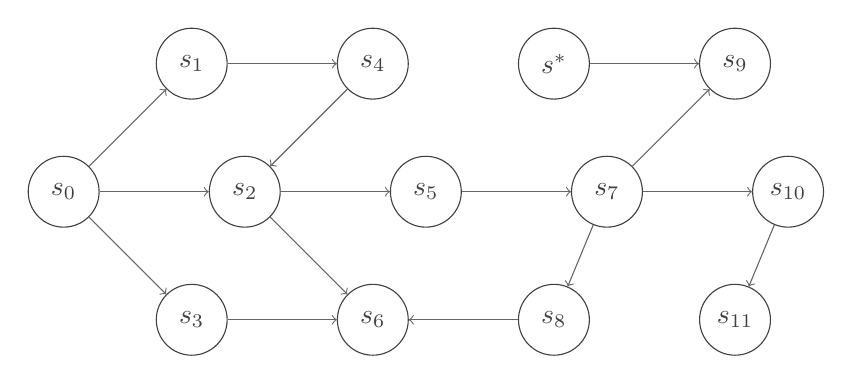
\begin{tikzpicture}[every node/.style={circle, draw}, node distance=23mm, minimum size=9mm]
        \node[color=black!75] (s0) {$s_0$};
        \node[right of=s0, color=black!75] (s1) {$s_2$};
        \node[below right of=s0, color=black!75] (s2) {$s_3$};
        \node[above right of=s1, color=black!75] (s3) {$s_4$};
        \node[right of=s1, color=black!75] (s4) {$s_5$};
        \node[right of=s2, color=black!75] (s5) {$s_6$};
        \node[right of=s3, color=black!75] (s6) {$s^*$};
        \node[right of=s4, color=black!75] (s7) {$s_7$};
        \node[right of=s5, color=black!75] (s8) {$s_8$};
        \node[right of=s6, color=black!75] (s9) {$s_9$};
        \node[above right of=s0, color=black!75] (s10) {$s_1$};
        \node[right of=s7, color=black!75] (s11) {$s_{10}$};
        \node[right of=s8, color=black!75] (s12) {$s_{11}$};

        \draw[->, color=black!60] (s0) -- (s1);
        \draw[->, color=black!60] (s0) -- (s2);
        \draw[->, color=black!60] (s3) -- (s1);
        \draw[->, color=black!60] (s1) -- (s4);
        \draw[->, color=black!60] (s2) -- (s5);
        \draw[->, color=black!60] (s10) -- (s3);
        \draw[->, color=black!60] (s4) -- (s7);
        \draw[->, color=black!60] (s7) -- (s8);
        \draw[->, color=black!60] (s8) -- (s5);
        \draw[->, color=black!60] (s6) -- (s9);
        \draw[->, color=black!60] (s7) -- (s9);
        \draw[->, color=black!60] (s0) -- (s10);
        \draw[->, color=black!60] (s7) -- (s11);
        \draw[->, color=black!60] (s11) -- (s12);
        \draw[->, color=black!60] (s1) -- (s5);
      \end{tikzpicture}
\end{figure}

To exemplify, Figure~\ref{fig:statespace} presents a state space. BFS starts by expanding the initial state $s_0$, and then expands $s_1$, $s_2$ and $s_3$. In sequence, it expands the successor of $s_1$ ($s_4$), then of $s_2$ ($s_5$ and $s_6$), and so on until a solution is found. On the other hand, DFS expands the initial state $s_0$ and continues expanding a newly generated successor until it reaches a solution or a state without successors (e.g., $s_6$), at which point the algorithm backtracks to the nearest state that has an unvisited successor and continues the search.

Blind search algorithms are not suitable for solving planning tasks due to their inherent limitations in efficiently exploring the search space, and instead, heuristic search is employed, which will be introduced in the next section. However, BFS and DFS can still be valuable as sampling algorithms in planning. By sampling the search space using these algorithms, we can selectively focus on regions that are either closer to the initial state, using BFS, or more distant, using DFS.

\section{Heuristic Search}
\label{sec:background_heuristicsearch}

Exploring a large portion of the search space to finding a plan can quickly become computationally infeasible, especially for complex planning domains with large state spaces. Therefore, the primary technique for solving planning tasks is heuristic search. Heuristic search algorithms address this challenge by utilizing heuristics, which are approximate measures of distance or cost, to guide the search towards promising regions of the search space. These heuristics estimate how close a given state is to the goal state and provide guidance on which actions to prioritize during the search.

A commonly used heuristic search algorithm in classical planning is \astar search. \astar combines the cost of reaching a state from the initial state ($g$-value) with a heuristic estimate of the remaining cost to reach the goal state ($h$-value). The heuristic estimate is also known as the cost-to-goal estimate. By considering both the past cost and the estimated future cost, \astar can efficiently explore the search space and find a solution.

Greedy Best-First Search (GBFS) is another widely used heuristic search algorithm in classical planning. It is a variant of \astar search that prioritizes expanding states with the lowest heuristic values, without considering the past cost of reaching those states. GBFS is considered a ``greedy'' algorithm because it only takes into account the heuristic estimate and makes decisions solely based on that information. While GBFS can be extremely efficient in terms of exploration speed, it does not guarantee finding an optimal solution. The lack of considering the past cost can lead to suboptimal solutions or even failure to find a solution in some cases. Nonetheless, GBFS remains a popular choice in planning tasks where finding any feasible solution quickly is more important than finding the optimal solution. Therefore, for our experiments, GBFS will serve as the search algorithm.

\subsection{Heuristic Functions}
\label{sec:background_heuristicfunctions}

The effectiveness of heuristic search relies heavily on the quality of the heuristic function used. A heuristic function~$h:\mathcal{S}\rightarrow\R_{+}\cup\{\infty\}$ maps each state in the state space~$\mathcal{S}$ to a non-negative number or infinity. The number represents the cost-to-goal estimate ($h$-value) for the given state. An infinity value indicates that the state is a dead-end, i.e., it does not have any path to the goal. A heuristic function is more efficient when its $h$-value closely approximate the true goal distance. The optimal heuristic function \hstar consistently produces the cost of an optimal plan for all state~$s \in \mathcal{S}$.

Heuristic function possesses certain properties such as admissibility and consistency. Admissibility refers to the characteristic of a heuristic function that never overestimates the true goal distance. An admissible heuristic ensures that the search algorithm explores the most promising paths and guarantees optimality when combined with certain search algorithms such as \astar. Still, a heuristic function is consistent if the estimated cost of a state is always less than or equal to the sum of the estimated cost to reach a successor plus the cost of the action.

Heuristics can be arbitrary functions, allowing for flexibility in designing and customizing based on domain knowledge and problem-specific insights. Based on this, a heuristic can be classified as either model-based or model-free. In a model-free setting where we interact with the planning task only by functions that allow accessing the initial state~$s_0$, the goal condition~$s^*$, and the successors $\sucs(s)$ of a state $s$. In this setting, we do not have access to the logical description of operators, we only have access to black-box functions~\cite{Sturtevant2019} -- which could also be learned -- that, given a state, returns its successors and predecessors. Note that this setting is also used in reinforcement learning. Some approaches also provide access to each variable's domain. In contrast, a model-based heuristic uses the complete description of the model, which permits, for example, reasoning about operators and the computation of mutexes.

An example of a model-based heuristic is the FF~(Fast Forward) heuristic~\cite{Hoffmann.Nebel/2001}, which computes its cost-to-goal estimates by considering the relaxed version of the planning problem. In the relaxed version, all preconditions and delete effects of the operators are ignored, resulting in a simplified version of the problem. The FF heuristic extracts a solution from the relaxed version and computes the number of actions in the plan, using it as the cost-to-goal estimate. On the other hand, the goal-count is a model-free heuristic that does not rely on the planning model. Instead, it counts the number of unsatisfied goal conditions in the current state, assuming that each unsatisfied condition requires an additional operator to be satisfied. Both the FF and goal-count heuristics are evaluated in Chapter~\ref{sec:experiments}.

\section{Neural Networks}
\label{sec:background_neuralnetworks}

Neural networks (NN) have gained significant popularity due to their ability to learn and generalize from complex datasets. In classical planning, various approaches using neural networks have been proposed (see Section~\ref{sec:background_relatedwork}). These approaches range from simpler models that prioritize processing speed -- and consequently, expansion rate -- to more complex architectures that exploit the relational structure of a domain.

\begin{figure}[ht]
    \caption{The structure of the artificial neuron.}
    \label{fig:neuron}
    \centering
    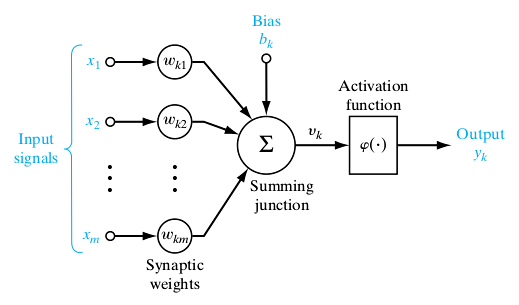
\includegraphics[width=0.9\linewidth]{figures/neuron.png} \\
    Source:~\cite{Haykin/2009}
\end{figure}

At the core of a neural network are individual artificial neurons, illustrated in Figure~\ref{fig:neuron}. A neuron consists of three main components: input signals, weights, and an activation function. Each neuron receives input from the previous layer or directly from the input data. These inputs are weighted, representing the importance of each input, and combined with a bias term. The result value are then passed through an activation function, which introduces non-linearity and determines the output of the neuron. One example of an activation function is the Rectified Linear Unit (ReLU) activation, which returns the input if it is positive and zero otherwise.

Neurons are combined to form layers in a neural network. Each layer serves a specific purpose in processing and transforming the input data. The input layer directly receives the input data and passes it to the subsequent layers. The hidden layers, located between the input and output layers, are responsible for extracting and learning higher-level features from the input. These hidden layers enable the network to capture complex patterns and relationships within the data. Finally, the output layer produces the prediction for the given input. A specific type of neural network called a feedforward neural network (FNN) operates by allowing information to flow in one direction, from the input layer through the hidden layers to the output layer. When a neural network has multiple hidden layers, it is referred to as a deep neural network.

The learning process involves adjusting the network's parameters, such as weights and biases, to minimize the error between its predictions and the true values of the training samples. This adjustment is typically performed using an optimization algorithm to minimize a specified loss function. One commonly used loss function is the Mean Squared Error (MSE) loss function, which quantifies the error by calculating the average squared difference between the predicted and true values. For a more comprehensive understanding of the weight adjustment and training process in neural networks, Haykin (\citeyear{Haykin/2009}) provides in-depth insights.

To efficiently update the parameters, training is often performed on batches of data rather than individual samples. The batch size determines the number of training examples that are processed together before updating the network's parameters. Larger batch sizes can lead to more stable updates but require more memory and computation, while smaller batch sizes may result in more frequent updates but with higher variance.

By iteratively adjusting its parameters based on the training data, a neural network gradually improves its ability to make accurate predictions. The quality of the neural network heavily relies on the quality and diversity of the training samples used during the learning process. Additionally, the network's capacity to learn and generalize from the training data is influenced by its structural characteristics. A well-designed and appropriately structured neural network enhances learning efficiency and improves its ability to handle complex patterns and relationships within the data.

\subsection{Residual Networks}
\label{sec:background_resnets}

ResNet, short for Residual Network, was proposed by He et al.~(\citeyear{He.etal/2016}) and has gained significant attention due to its ability to address the vanishing gradient problem~\cite{Hochreiter/1998} and improve training performance for deep neural networks. While its initial success was in the field of image recognition, ResNet has also been investigated in the context of planning~\cite{Agostinelli.etal/2019,Ferber.etal/2022} as a means to address training deep neural networks.

ResNet introduces the concept of residual connections or skip connections, which enable the network to learn residual mappings. These connections allow the network to bypass certain layers and pass the input directly to deeper layers. By doing so, ResNet mitigates the degradation problem that can occur in very deep networks, where adding more layers leads to decreased accuracy. The residual connections help preserve information and facilitate the flow of gradients during the training process.

\begin{figure}[ht]
    \caption[A regular block and a residual block.]{A regular block (left) and a residual block (right).}
    \label{fig:residual_block}
    \addvspace{\baselineskip}
    \centering
    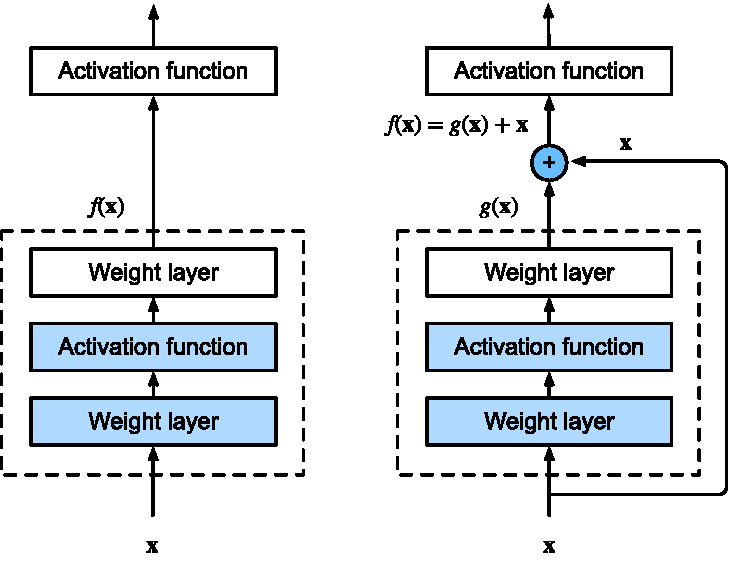
\includegraphics[width=0.75\linewidth]{figures/residual_block.pdf} \\
    Source:~\cite{Zhang.etal/2021}
\end{figure}

The Figure~\ref{fig:residual_block} illustrates a schematic representation of both a regular block and a residual block, with a shortcut connection that skips one layer, in a ResNet architecture. In a regular block, the output of its layers is directly mapped to the activation function. On the other hand, in a residual block, the network needs to learn the residual mapping $g(x)=f(x)-x$, making it easier for the network to optimize the model's performance. He et al.~(\citeyear{He.etal/2016}) provides a more detailed understanding of the ResNets.

\section{Learning Heuristic Functions with Neural Networks}
\label{sec:background_learningheuristics}

Many heuristics for classical planning are derived from a model of the task, such as the \sas model introduced in this chapter. An obvious alternative is to learn to map a state $s$ to its heuristic value $h(s)$. We focus here on learning with NNs, although other supervised learning methods could be used. To learn a heuristic function, an NN is trained on pairs of states~$s$ and cost-to-goal estimates~$c$. The learned heuristic functions are usually not admissible, so traditional optimality guarantees are lost.

A propositional representation of a state is more suitable for learning functions over states. To this end, consider a planning task $\Pi=\langle\mathcal{V},\mathcal{O},s_0,s^*, \text{cost}\rangle$, and let $\mathcal{V}=\{v_1,\ldots,v_n\}$ and $D(v_i)=\{d_{i1},\ldots,d_{i,s_i}\}$, $i\in[n]$ be some order of the variables and their domains. We represent any state $s$ by a sequence of facts $$\mathcal{F}(s)=(f_{11},f_{12},\ldots,f_{1,s_1},\ldots,f_{n1},f_{n2},\ldots,f_{n,s_n}),$$ where each fact $f_{ij}=[s(v_i)=d_{ij}]$ indicates if variable $v_i$ assumes value $d_{ij}$ in state $s$. Note that facts $\mathcal{F}_i=\{f_{i1},\ldots,f_{i,s_i}\}$ corresponding to variable $v_i$ satisfy the consistency condition $\sum_{f\in \mathcal{F}_i} f\leq 1$ since each variable assumes at most one value, and $\sum_{f\in \mathcal{F}_i} f=0$ only if $v_i$ is undefined. More generally, for any set of facts $\mathcal{F}$ we write $\mutex(\mathcal{F})$ if $\sum_{f\in \mathcal{F}} [f]\leq 1$ must be satisfied in states of $\Pi$. Many planning systems can deduce mutexes from the description of the planning task $\Pi$~\cite{Helmert/2009}; we will discuss and analyze their utility for sampling states later. Some architectures provide additional input to the NN, e.g.,~the propositional representation of the goal condition. The target output for training may be the cost-to-goal estimates directly or some encoding of them.

An important aspect of sample generation related to challenges C1 and C2 (Section \ref{sec:intro}) is the degree of dependency on the domain model -- ideally, we would like to learn in a model-free setting -- or the planning task and the cost of generating the samples. The cost of sample generation depends on the number of samples and the cost to generate each. This generates the problem of deciding how many samples are required, although in general, only a very small part of the state space can be sampled. More importantly, ideal samples would be labeled with the perfect heuristic $h^*$, which maps each state~$s$ to the cost of an optimal $s$-plan or $\infty$ if no such plan exists. In general, ideal labeling is impractical since it requires solving the planning task on a large number of initial states. Therefore, we are mainly interested in good heuristic estimates that can be generated fast. We analyze the influence of sample size and quality experimentally later.

Additionally, and related to challenges C3 and C4, network architecture and sample generation depends on the range of tasks the learner intends to generalize. This may be the state space of a planning task, a planning domain, or an entire planning formalism. In the first case, the set of planning tasks is defined over any pair of initial state $s_0$ and goal $s^*$. Often the set of planning tasks is restricted to select the initial state from the \fssp of some given initial state and to a fixed goal. In the second case, the learned function has to generalize over all domain tasks. Finally, a learning-based heuristic that generalizes over a planning formalism is domain-independent. An important aspect of sample generation is the distribution of states part of the sample set. For example, the sample set can contain only states with a short distance to the goal or only states with a short distance to the initial states. In this dissertation, the distribution of states describes how often each \hstar-value occurs in the sample set.

\section{Related Work}
\label{sec:background_relatedwork}

There have been two main research foci on learning heuristic functions. The first uses strongly model-based approaches to generate samples and aims to generalize over domains or a planning formalism. The second uses partially model-based approaches to generate samples and aims to generalize only over a state space. We describe these approaches as partially model-based because they only use the model to identify mutexes.

\subsection{Strongly Model-Based}

The usual setting for the first set of approaches~\cite{Toyer.etal/2018,Shen.etal/2020,Toyer.etal/2020,Gehring.etal/2022,Stahlberg.etal/2022} is to train a structured NN with samples of small tasks of a domain generated with a strongly model-based method and evaluated on larger tasks of the same domain. The structured networks trained can be general networks such as neural logic machines~\cite{Dong.etal/2018} and graph neural networks~\cite{Gori.etal/2005,Scarselli.etal/2008}

In the context of planning, Shen et al.~(\citeyear{Shen.etal/2020}) introduced hypergraph neural networks (HGN) as an extension of graph networks~\cite{Battaglia.etal/2018}. HGN aims to learn planning heuristics through training, with a particular focus on developing domain-independent heuristics capable of generalizing across various domains, as well as domain-specific and multi-domain heuristics. HGN encompasses vertices representing task propositions within a hypergraph structure, with edges denoting actions connecting the preconditions to their effects. The network learns latent features directly from the hypergraph representation of the planning problem.

Another approach proposed explicitly for planning tasks is the Action Schema Networks (ASNet)~\cite{Toyer.etal/2018}. ASNets are composed of alternating proposition and action layers, with the first and last layer always being an action layer. Each action layer contains an action module for each action in a specific task, while each propositional layer contains a proposition module for each proposition in the task. Weight sharing is employed to optimize efficiency, where action modules with actions derived from the same action schema share the same weight, and proposition modules with propositions derived from the same predicate share the same weight. This weight sharing allows for the reuse of a single set of learned weights across all tasks within a class of planning problems.

These networks require the logical description of the domain and the task to be instantiated and can generalize well, with competitive results compared to logic-based heuristics. These approaches also help in understanding learning heuristics. For example, the main goal of St\aa hlberg et al.~(\citeyear{Stahlberg.etal/2022}) is to understand the expressive power and limitations of learning heuristics. The main limitation of these approaches is the strong dependence on the domain model and task description.

\subsection{Partially Model-Based}

The second set of approaches~\cite{Ferber.etal/2020a, Yu.etal/2020, Ferber.etal/2022, OToole/2022} typically trains an FNN and evaluates the learned heuristic on a state space using tasks with the same goal and different initial states. These networks are trained with pairs of states and cost-to-goal estimates. In this setting, Ferber et al.~(\citeyear{Ferber.etal/2020a}) systematically study hyperparameters on the architecture of the FNN and found that their influence is secondary. They found that for a fixed architecture, two aspects significantly influence how informed the heuristic is: the subset of selected samples and the size of the sample set. 

Ferber et al.~(\citeyear{Ferber.etal/2022}) uses a combination of backward and forward searches~\cite{Arfaee.etal/2011}. First, it generates new initial states with backward random walks and then solves them with a GBFS guided by a learned heuristic. The sampling is performed in parallel with the training, and the number of samples per search varies throughout the process. Initially, it starts with a random value ranging from $0$ to $5$, and it doubles as plans are found. The plans found provide the samples for the next training epoch, where each sample is a state in the plan with the cost-to-goal estimate as its distance to the goal. Their FNN architecture is a ResNet with two hidden layers and a residual block consisting of two hidden layers.

O'Toole et al.~(\citeyear{OToole/2022}) uses the same FNN architecture as Ferber et al.~(\citeyear{Ferber.etal/2022}), which is also employed in this dissertation. They employ random walks to perform $5$ backward searches from the goal, with a depth of $500$, where the depth at which the state is generated serves as a cost-to-goal estimate. Subsequently, each sampled partial state is converted into $20$ complete states and added to the sample set. Additionally, they sample an additional $50$\,K randomly generated states with high cost-to-goal estimates, resulting in a total of $100$\,K samples. They showed that random sampling significantly improves the performance of the heuristic function.

Yu et al.~(\citeyear{Yu.etal/2020}) employed a backward search approach using the DFS algorithm. In their best configuration, they perform $800$ searches, each limited to $500$ samples. Thus, their sample set comprises $400$\,K states, with the depth at which each state was generated serving as a cost-to-goal estimate. In contrast to the previous approaches, they use a compact FNN consisting of only one hidden layer with $16$ neurons.

The methods from the partially model-based approaches are highly independent of the domain model and planning task description and require low computational resources to generate samples and train the FNN. However, they suffer from high performance variability, given the FNN initialization and the sample set used. Also, despite having competitive results compared to logic-based heuristics, they are still unable to surpass the goal-count heuristic.
